% Figure 7 of "Galashin's Conjecture 4.3 via a convex gradient": the crossing graph in winding-one cycles and the Hessian assembled from them.
% Source of the figure, typeset in the paper's own fonts (T1, Latin Modern, 11pt) at the paper's text
% width (6.5in), so \includegraphics does not rescale it. Illustrates CLH-3 and CLH-5; it adds no assertion.
% Build: pdflatex <this file> && pdftocairo -svg <this file>.pdf <this file>.svg
\documentclass[11pt]{standalone}
\usepackage[T1]{fontenc}
\usepackage{lmodern}
\usepackage{amsmath,amssymb}
\usepackage{tikz}
\usetikzlibrary{arrows.meta,positioning,calc}

% the palette of the paper's other figures: blue solid for the first strand or arc, ochre dashed for the second
\definecolor{ink}{HTML}{233740}
\definecolor{muted}{HTML}{65757D}
\definecolor{pblue}{HTML}{0072B2}
\definecolor{qochre}{HTML}{B87827}

\tikzset{
  base/.style={draw=muted, line width=0.5pt},
  exit/.style={circle, draw=ink, fill=white, line width=0.6pt, inner sep=0pt, minimum size=4.6pt},
  entry/.style={circle, draw=ink, fill=ink, line width=0.6pt, inner sep=0pt, minimum size=4.6pt},
  exitP/.style={exit, draw=pblue}, entryP/.style={entry, draw=pblue, fill=pblue},
  exitQ/.style={exit, draw=qochre}, entryQ/.style={entry, draw=qochre, fill=qochre},
  strandP/.style={pblue, line width=1.1pt, -{Stealth[length=5pt,width=4.2pt]}, shorten >=2.4pt},
  strandQ/.style={qochre, line width=1.1pt, dash pattern=on 4pt off 1.6pt, -{Stealth[length=5pt,width=4.2pt]}, shorten >=2.4pt},
  lab/.style={font=\footnotesize, inner sep=1.2pt, text=ink},
  labm/.style={font=\small, inner sep=1.2pt, text=ink},
  labP/.style={font=\small, inner sep=1.2pt, text=pblue},
  labQ/.style={font=\small, inner sep=1.2pt, text=qochre},
  muted text/.style={text=muted},
  ttl/.style={font=\small, text=ink, inner sep=0pt},
  negE/.style={font=\small, text=pblue, inner sep=0pt},
  posE/.style={font=\small, text=qochre, inner sep=0pt},
  zeroE/.style={font=\small, text=ink, inner sep=0pt},
  idx/.style={font=\footnotesize, text=muted, inner sep=0pt},
}
\tikzset{
  vtx/.style={circle, draw=ink, fill=white, line width=0.6pt, inner sep=0pt, minimum size=0.62cm, font=\small, text=ink},
  cycP/.style={pblue, line width=1.2pt, -{Stealth[length=5.5pt,width=4.5pt]}, shorten >=1pt, shorten <=1pt},
  cycQ/.style={qochre, line width=1.2pt, dash pattern=on 4pt off 1.6pt, -{Stealth[length=5.5pt,width=4.5pt]}, shorten >=1pt, shorten <=1pt},
  sec/.style={font=\small, text=ink, inner sep=0pt, anchor=west},
  frm/.style={font=\small, text=ink, inner sep=0pt},
  fn/.style={font=\footnotesize, text=ink, inner sep=0pt, anchor=north west, align=flush left},
  stepn/.style={font=\footnotesize, text=ink, inner sep=1.5pt},
  aux/.style={muted, line width=0.8pt, -{Stealth[length=5pt,width=4pt]}},
}

\begin{document}
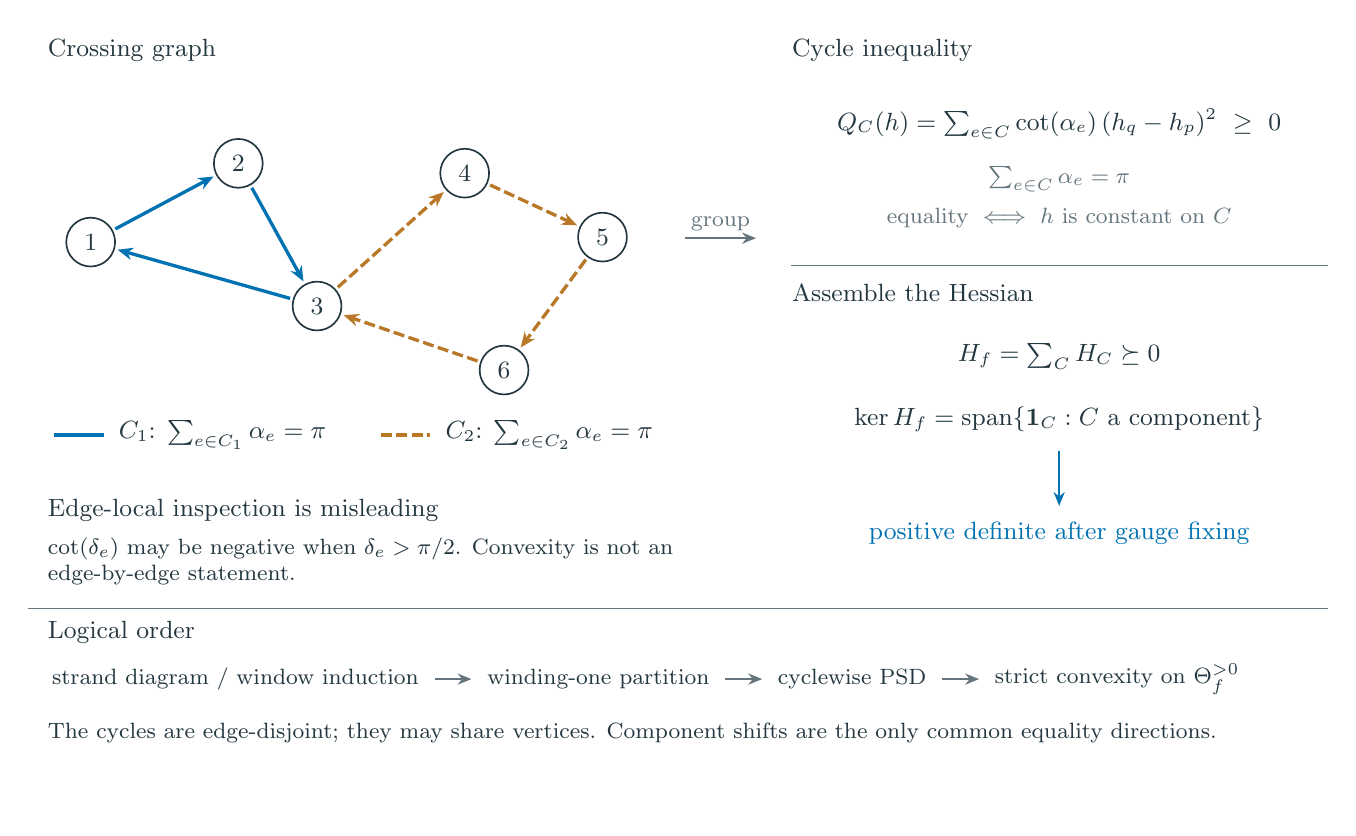
\begin{tikzpicture}[x=1cm,y=1cm]
\useasboundingbox (-0.25000,-9.73300) rectangle (16.26000,0.17300);
\node[sec] at (0.0,-0.12) {Crossing graph}; %t sec-graph
\node[vtx] (v1) at (0.550,-2.550) {1}; %t vertex1
\node[vtx] (v2) at (2.425,-1.550) {2}; %t vertex2
\node[vtx] (v3) at (3.425,-3.362) {3}; %t vertex3
\node[vtx] (v4) at (5.300,-1.675) {4}; %t vertex4
\node[vtx] (v5) at (7.050,-2.487) {5}; %t vertex5
\node[vtx] (v6) at (5.800,-4.175) {6}; %t vertex6
\draw[cycP] (v1) -- (v2); %c C1 1,2
\draw[cycP] (v2) -- (v3); %c C1 2,3
\draw[cycP] (v3) -- (v1); %c C1 3,1
\draw[cycQ] (v3) -- (v4); %c C2 3,4
\draw[cycQ] (v4) -- (v5); %c C2 4,5
\draw[cycQ] (v5) -- (v6); %c C2 5,6
\draw[cycQ] (v6) -- (v3); %c C2 6,3
\draw[cycP, -] (0.050,-5.000) -- (0.750,-5.000); %k C1
\node[frm, anchor=west] at (0.900,-5.000) {$C_{1}$: $\sum_{e\in C_{1}}\alpha_e=\pi$}; %t tag1
\draw[cycQ, -] (4.200,-5.000) -- (4.900,-5.000); %k C2
\node[frm, anchor=west] at (5.050,-5.000) {$C_{2}$: $\sum_{e\in C_{2}}\alpha_e=\pi$}; %t tag2
\node[sec] at (0.0,-5.95) {Edge-local inspection is misleading}; %t sec-local
\node[fn, text width=8.0cm] at (0.0,-6.3) {$\cot(\delta_e)$ may be negative when $\delta_e>\pi/2$. Convexity is not an edge-by-edge statement.}; %t local
\draw[aux] (8.1,-2.5) -- (9.0,-2.5); %a group
\node[font=\footnotesize, text=muted, anchor=south, inner sep=1pt] at (8.55,-2.45) {group}; %t group
\node[sec] at (9.45,-0.12) {Cycle inequality}; %t sec-cycle
\node[frm] at (12.850,-1.05) {$Q_C(h)=\sum_{e\in C}\cot(\alpha_e)\,(h_q-h_p)^2\ \ge\ 0$}; %t qc
\node[font=\footnotesize, text=muted, inner sep=0pt] at (12.850,-1.75) {$\sum_{e\in C}\alpha_e=\pi$}; %t sumalpha
\node[font=\footnotesize, text=muted, inner sep=0pt] at (12.850,-2.25) {equality $\iff$ $h$ is constant on $C$}; %t equality
\draw[muted, line width=0.4pt] (9.45,-2.85) -- (16.260,-2.85);
\node[sec] at (9.45,-3.2) {Assemble the Hessian}; %t sec-hessian
\node[frm] at (12.850,-4.0) {$H_f=\sum_C H_C\succeq 0$}; %t hf
\node[frm] at (12.850,-4.8) {$\ker H_f=\operatorname{span}\{\mathbf 1_C : C\text{ a component}\}$}; %t ker
\draw[aux, pblue] (12.850,-5.2) -- (12.850,-5.9); %a down
\node[frm, text=pblue] at (12.850,-6.25) {positive definite after gauge fixing}; %t posdef
\draw[muted, line width=0.4pt] (-0.250,-7.2) -- (16.260,-7.2);
\node[sec] at (0.0,-7.5) {Logical order}; %t sec-order
\node[stepn, anchor=west] (l1) at (0.0,-8.1) {strand diagram / window induction}; %t l1
\node[stepn, right=0.75cm of l1] (l2) {winding-one partition}; %t l2
\draw[aux, shorten <=4pt, shorten >=4pt] (l1.east) -- (l2.west); %a l1-l2
\node[stepn, right=0.75cm of l2] (l3) {cyclewise PSD}; %t l3
\draw[aux, shorten <=4pt, shorten >=4pt] (l2.east) -- (l3.west); %a l2-l3
\node[stepn, right=0.75cm of l3] (l4) {strict convexity on $\Theta_f^{>0}$}; %t l4
\draw[aux, shorten <=4pt, shorten >=4pt] (l3.east) -- (l4.west); %a l3-l4
\node[fn, text width=16.3cm] at (0.0,-8.65) {The cycles are edge-disjoint; they may share vertices. Component shifts are the only common equality directions.}; %t cycles-note
\end{tikzpicture}
\end{document}
